\documentclass[11pt,a4paper]{article}

% ============================================================
% Preamble
% ============================================================
\usepackage[utf8]{inputenc}
\usepackage[T1]{fontenc}
\usepackage{lmodern}
\usepackage[margin=1in]{geometry}
\usepackage{amsmath,amssymb,amsfonts}
\usepackage{graphicx}
\usepackage{booktabs}
\usepackage{hyperref}
\usepackage{cleveref}
\usepackage{algorithm}
\usepackage{algorithmic}
\usepackage{enumitem}
\usepackage{xcolor}
\usepackage{tikz}
\usetikzlibrary{shapes,arrows,positioning,fit}
\usepackage{float}
\usepackage{subcaption}
\usepackage{multirow}
\usepackage{tabularx}
\usepackage{fancyhdr}
\usepackage{authblk}
\usepackage{abstract}
\usepackage{natbib}
\bibliographystyle{plainnat}

\hypersetup{
    colorlinks=true,
    linkcolor=blue!70!black,
    citecolor=green!50!black,
    urlcolor=blue!80!black
}

\pagestyle{fancy}
\fancyhf{}
\rhead{Zoo Labs Foundation}
\lhead{Zoo Data Commons}
\rfoot{Page \thepage}

% ============================================================
\title{\textbf{Zoo Data Commons: A Decentralized Repository for Open Biodiversity Datasets} \\[0.5em]
\large FAIR-Compliant Data Infrastructure with Provenance Tracking and Incentivized Curation}

\author[1]{Zoo Labs Foundation Research}
\affil[1]{Zoo Labs Foundation, Research Division \\ \texttt{research@zoo.ngo}}

\date{February 2026}

\begin{document}
\maketitle

% ============================================================
% Abstract
% ============================================================
\begin{abstract}
\noindent
Biodiversity data is fragmented across thousands of institutional repositories, government databases, citizen science platforms, and individual researcher collections, impeding the large-scale ecological analyses essential for conservation decision-making.
We present the Zoo Data Commons (ZDC), a decentralized repository for open biodiversity datasets built on IPFS and the Zoo Network blockchain.
ZDC introduces a novel \emph{Data Object Model} that wraps biodiversity datasets in cryptographically signed metadata envelopes conforming to the FAIR principles (Findable, Accessible, Interoperable, Reusable).
Each data object carries an immutable provenance chain recording its complete transformation history from raw collection through processing, validation, and aggregation.
We implement a three-tier access control system supporting open, permissioned, and sovereign data governance models, enabling indigenous communities and local stakeholders to maintain control over culturally sensitive ecological knowledge.
A token-incentivized curation market rewards data contributors, validators, and annotators, aligning individual incentives with collective data quality improvement.
Over 12 months of operation, ZDC has ingested 2.4 million biodiversity records across 14,200 species from 847 contributors, with a median data quality score 23\% higher than comparable centralized repositories.
The platform has facilitated 312 cross-institutional data reuse events and supported 47 peer-reviewed publications.
ZDC is specified as Zoo Improvement Proposal ZIP-009 and deployed as open infrastructure.
\end{abstract}

\vspace{0.5em}
\noindent\textbf{Keywords:} biodiversity data, FAIR principles, decentralized storage, data provenance, IPFS, access control, open science

% ============================================================
% 1. Introduction
% ============================================================
\section{Introduction}
\label{sec:introduction}

Biodiversity data underpins conservation science, policy, and action.
Species occurrence records, population estimates, habitat maps, genetic sequences, and ecological interaction networks collectively form the empirical foundation for understanding and responding to the biodiversity crisis \citep{diaz2019global}.
Yet this data ecosystem suffers from chronic fragmentation, inconsistent quality, and misaligned incentives that severely limit its utility.

The Global Biodiversity Information Facility (GBIF) aggregates over 2.4 billion occurrence records from 1,800 institutions \citep{gbif2024overview}, representing the most ambitious centralized aggregation effort.
Despite its success, GBIF faces structural limitations: metadata quality varies enormously across providers, provenance tracking is limited to institutional attribution, temporal coverage is biased toward recent decades and temperate regions, and the centralized architecture creates governance challenges around data sovereignty and access control \citep{yesson2007how}.

The FAIR principles---Findable, Accessible, Interoperable, Reusable---articulate the requirements for scientific data to support automated discovery and reuse \citep{wilkinson2016fair}.
However, surveys consistently find that fewer than 20\% of biodiversity datasets fully satisfy FAIR criteria \citep{jacobsen2020fair}, primarily due to inadequate metadata, inconsistent formats, and absence of machine-readable provenance.

We present the Zoo Data Commons (ZDC), a decentralized biodiversity data repository that addresses these challenges through three technical contributions:

\begin{enumerate}[leftmargin=*]
    \item \textbf{FAIR-Native Data Object Model:} A self-describing data object format that embeds rich, machine-readable metadata including taxonomic ontology mappings, spatial reference systems, temporal resolution, and collection methodology descriptors (\Cref{sec:data_model}).
    \item \textbf{Provenance-Preserving Storage:} A content-addressed storage architecture on IPFS with blockchain-anchored provenance chains that record the complete transformation history of every dataset (\Cref{sec:storage}).
    \item \textbf{Sovereign Access Control:} A three-tier access governance framework supporting open, permissioned, and sovereign data models, enabling data holders to define and enforce nuanced sharing policies (\Cref{sec:access}).
\end{enumerate}

% ============================================================
% 2. Related Work
% ============================================================
\section{Related Work}
\label{sec:related}

\subsection{Biodiversity Data Infrastructure}

The global biodiversity data landscape comprises several major platforms.
GBIF provides a centralized index of species occurrence records with standardized Darwin Core format \citep{wieczorek2012darwin}.
The Integrated Digitized Biocollections (iDigBio) focuses on museum specimen digitization \citep{nelson2019digitization}.
OBIS (Ocean Biogeographic Information System) specializes in marine biodiversity data \citep{grassle2000ocean}.
GenBank and BOLD provide genetic sequence repositories \citep{benson2018genbank}.

These platforms operate as centralized aggregators: data providers push records to central servers that maintain authoritative copies.
This architecture creates well-known problems of data staleness, attribution erosion, and governance concentration \citep{arinoetal2013}.

\subsection{FAIR Data Principles}

The FAIR principles have become the de facto standard for scientific data management \citep{wilkinson2016fair}.
Implementation frameworks include FAIRsFAIR metrics \citep{devaraju2021fairsfair}, GO-FAIR implementation networks, and FAIR Digital Object architectures \citep{schultes2019fair}.
However, most FAIR implementations are retrospective assessments of existing data rather than architecturally enforced properties.

\subsection{Decentralized Data Systems}

IPFS (InterPlanetary File System) provides content-addressed storage with deduplication and peer-to-peer distribution \citep{benet2014ipfs}.
Filecoin extends IPFS with economic incentives for persistent storage \citep{protocol2017filecoin}.
Ocean Protocol implements a decentralized data marketplace with compute-to-data capabilities \citep{mcconaghy2020ocean}.
\citet{ramachandran2018trinity} proposed blockchain-based data provenance for healthcare, demonstrating the pattern we extend to biodiversity data.

\subsection{Indigenous Data Sovereignty}

The CARE Principles for Indigenous Data Governance (Collective Benefit, Authority to Control, Responsibility, Ethics) complement FAIR by centering the rights and interests of indigenous peoples in data management \citep{carroll2020care}.
Traditional Knowledge (TK) labels provide a mechanism for indigenous communities to express culturally appropriate access conditions \citep{anderson2010tk}.
ZDC's sovereign access tier directly implements these principles.

% ============================================================
% 3. Data Object Model
% ============================================================
\section{FAIR-Native Data Object Model}
\label{sec:data_model}

\subsection{Object Structure}

A Zoo Data Object (ZDO) is the atomic unit of the Data Commons.
Each ZDO comprises four components:

\begin{equation}
    \text{ZDO} = (\mathcal{M}, \mathcal{D}, \mathcal{P}, \mathcal{G})
\end{equation}

\noindent where $\mathcal{M}$ is the metadata envelope, $\mathcal{D}$ is the data payload, $\mathcal{P}$ is the provenance chain, and $\mathcal{G}$ is the governance specification.

\subsection{Metadata Envelope}

The metadata envelope $\mathcal{M}$ is a structured document conforming to a JSON-LD schema that extends Darwin Core with additional fields for FAIR compliance:

\begin{equation}
    \mathcal{M} = (\text{id}, \text{schema}, \text{taxon}, \text{spatial}, \text{temporal}, \text{method}, \text{quality}, \text{links})
\end{equation}

\begin{table}[H]
\centering
\caption{Metadata envelope fields and their FAIR mapping.}
\label{tab:metadata}
\begin{tabularx}{\textwidth}{@{}llcX@{}}
\toprule
\textbf{Field} & \textbf{Type} & \textbf{FAIR} & \textbf{Description} \\
\midrule
\texttt{id} & CID & F1 & Content-addressed identifier (IPFS CID) \\
\texttt{schema} & URI & I1 & Reference to the data schema definition \\
\texttt{taxon} & OntologyRef & I2 & Taxonomic classification with ontology mapping \\
\texttt{spatial} & GeoJSON & F3 & Geographic extent with coordinate reference system \\
\texttt{temporal} & ISO8601 & F3 & Temporal coverage with resolution specification \\
\texttt{method} & MethodRef & R1 & Collection methodology with controlled vocabulary \\
\texttt{quality} & QualityScore & R2 & Automated quality assessment scores \\
\texttt{links} & LinkSet & F4 & Related ZDOs, publications, and external resources \\
\bottomrule
\end{tabularx}
\end{table}

\subsection{Taxonomic Ontology Integration}

ZDC maintains a unified taxonomic knowledge graph that reconciles multiple backbone taxonomies:

\begin{equation}
    \mathcal{T}_{\text{unified}} = \text{Reconcile}(\mathcal{T}_{\text{GBIF}}, \mathcal{T}_{\text{ITIS}}, \mathcal{T}_{\text{CoL}}, \mathcal{T}_{\text{WoRMS}})
\end{equation}

The reconciliation algorithm produces a mapping $\phi: \mathcal{N}_{\text{source}} \rightarrow \mathcal{N}_{\text{unified}}$ from source taxonomy names to unified nodes, with confidence scores and conflict annotations.
Each ZDO's taxonomic field references a node in the unified graph, enabling cross-dataset queries that are invariant to naming conventions.

We use a graph embedding approach to detect synonyms and near-matches:

\begin{equation}
    \text{sim}(n_i, n_j) = \cos(\mathbf{e}_i, \mathbf{e}_j) + \lambda \cdot \text{Jaccard}(\text{features}(n_i), \text{features}(n_j))
\end{equation}

\noindent where $\mathbf{e}_i$ is the embedding of node $n_i$ from a graph neural network trained on the taxonomy structure, and $\text{features}(n_i)$ includes morphological, ecological, and geographic characteristics.

\subsection{Data Quality Assessment}

Each ZDO undergoes automated quality assessment producing a vector of scores:

\begin{equation}
    \mathbf{q} = (q_{\text{complete}}, q_{\text{consistent}}, q_{\text{spatial}}, q_{\text{temporal}}, q_{\text{taxonomic}})
\end{equation}

\begin{itemize}[leftmargin=*]
    \item $q_{\text{complete}} \in [0,1]$: Fraction of required metadata fields populated.
    \item $q_{\text{consistent}} \in [0,1]$: Internal consistency score (e.g., species range vs.\ reported coordinates).
    \item $q_{\text{spatial}} \in [0,1]$: Spatial precision and validity assessment.
    \item $q_{\text{temporal}} \in [0,1]$: Temporal precision and plausibility.
    \item $q_{\text{taxonomic}} \in [0,1]$: Confidence of taxonomic identification.
\end{itemize}

The composite quality score is:

\begin{equation}
    Q = \sum_{k} w_k \cdot q_k \cdot \mathbb{1}[q_k > q_k^{\min}]
\end{equation}

\noindent where $w_k$ are domain-specific weights and $q_k^{\min}$ are minimum thresholds; objects failing any threshold are flagged for review rather than rejected outright.

% ============================================================
% 4. Storage Architecture
% ============================================================
\section{Provenance-Preserving Storage}
\label{sec:storage}

\subsection{Content-Addressed Storage Layer}

ZDC uses IPFS for content-addressed storage of data objects.
Each ZDO is stored as a DAG of content-addressed blocks:

\begin{equation}
    \text{CID}(\text{ZDO}) = \text{hash}(\text{CID}(\mathcal{M}) \| \text{CID}(\mathcal{D}) \| \text{CID}(\mathcal{P}) \| \text{CID}(\mathcal{G}))
\end{equation}

This structure provides several properties:

\begin{enumerate}[leftmargin=*]
    \item \textbf{Deduplication:} Identical data payloads shared across ZDOs are stored once and referenced by CID.
    \item \textbf{Integrity:} Any modification to any component changes the root CID, making tampering detectable.
    \item \textbf{Selective Access:} Components can be retrieved independently; a user can access metadata without downloading the full data payload.
    \item \textbf{Versioning:} Updates produce new CIDs linked to previous versions through the provenance chain.
\end{enumerate}

\subsection{Persistence Layer}

IPFS provides availability only while content is pinned by at least one node.
ZDC ensures persistence through a multi-tier strategy:

\begin{table}[H]
\centering
\caption{Data persistence tiers.}
\label{tab:persistence}
\begin{tabularx}{\textwidth}{@{}lccX@{}}
\toprule
\textbf{Tier} & \textbf{Replicas} & \textbf{Duration} & \textbf{Mechanism} \\
\midrule
Hot & 5+ & Immediate & Zoo Network edge nodes with pinning incentives \\
Warm & 3+ & 1 year & Filecoin storage deals with verified miners \\
Cold & 1+ & 10 years & Institutional partnerships (museums, universities) \\
Archive & 1 & Permanent & Content hash anchored to Zoo blockchain \\
\bottomrule
\end{tabularx}
\end{table}

\subsection{Provenance Chain}

The provenance chain $\mathcal{P}$ records the complete transformation history of a ZDO:

\begin{equation}
    \mathcal{P} = [p_0, p_1, \ldots, p_n]
\end{equation}

\noindent where each provenance record $p_i$ is:

\begin{equation}
    p_i = (\text{action}_i, \text{agent}_i, \text{input}_i, \text{output}_i, \text{method}_i, t_i, \text{sig}_i)
\end{equation}

Actions include \texttt{COLLECT}, \texttt{DIGITIZE}, \texttt{TRANSFORM}, \texttt{VALIDATE}, \texttt{AGGREGATE}, \texttt{ANNOTATE}, and \texttt{DERIVE}.
The provenance chain is append-only and cryptographically linked: each record includes a hash of its predecessor, forming a hash chain anchored to the blockchain.

A formal provenance query language enables traversal:

\begin{equation}
    \text{Ancestors}(\text{ZDO}_k, \text{action}) = \{z : z \xrightarrow{\text{action}^*} \text{ZDO}_k\}
\end{equation}

This enables researchers to trace any derived result back to its raw collection events, answering questions such as ``what field observations contribute to this species distribution model?''

\subsection{Search and Discovery}

ZDC implements a federated search layer supporting spatial, temporal, taxonomic, and free-text queries:

\begin{equation}
    \text{Search}(R_{\text{spatial}}, T_{\text{temporal}}, \tau_{\text{taxon}}, q_{\text{text}}) \rightarrow \{\text{ZDO}_i : \text{match}(\text{ZDO}_i) > \theta\}
\end{equation}

The search index is maintained by Zoo Network nodes as a distributed hash table augmented with a spatial R-tree index and a taxonomic hierarchy index.
We use locality-sensitive hashing for approximate nearest-neighbor queries over embedding vectors derived from metadata and data content.

% ============================================================
% 5. Access Control
% ============================================================
\section{Sovereign Access Control}
\label{sec:access}

\subsection{Three-Tier Governance Model}

ZDC implements three access governance tiers reflecting the diversity of data sensitivity in biodiversity research:

\begin{table}[H]
\centering
\caption{Access governance tiers.}
\label{tab:access_tiers}
\begin{tabularx}{\textwidth}{@{}llX@{}}
\toprule
\textbf{Tier} & \textbf{Default Access} & \textbf{Use Cases} \\
\midrule
Open & Unrestricted & Published occurrence records, aggregated statistics, metadata \\
Permissioned & Request-based & Sensitive location data (endangered species), pre-publication data \\
Sovereign & Community-governed & Traditional ecological knowledge, indigenous land observations \\
\bottomrule
\end{tabularx}
\end{table}

\subsection{Permissioned Access}

Permissioned data uses attribute-based encryption (ABE) where the decryption key is conditioned on verifiable attributes of the requester:

\begin{equation}
    \text{Enc}(\mathcal{D}, \text{policy}) \rightarrow \text{CT}
\end{equation}

\begin{equation}
    \text{Dec}(\text{CT}, \text{key}_{\text{attributes}}) \rightarrow \begin{cases} \mathcal{D} & \text{if attributes satisfy policy} \\ \perp & \text{otherwise} \end{cases}
\end{equation}

Policies are expressed as Boolean formulas over attributes, such as:

\begin{verbatim}
    (role:researcher AND affiliation:university)
    OR (role:government AND jurisdiction:national)
    OR (approved-by:data-owner)
\end{verbatim}

\subsection{Sovereign Data Governance}

The sovereign tier implements the CARE Principles for Indigenous Data Governance \citep{carroll2020care}.
Each sovereign dataset is governed by a \emph{Data Governance Council} (DGC), a multisignature authority comprising community-designated representatives:

\begin{equation}
    \text{Access}(\text{ZDO}_{\text{sovereign}}) \leftarrow \text{Vote}_{\text{DGC}}(\text{request}) \geq \text{threshold}
\end{equation}

The DGC can:
\begin{itemize}[leftmargin=*]
    \item Set access policies with cultural context annotations (e.g., seasonal restrictions on sacred site data).
    \item Require benefit-sharing agreements as a condition of access.
    \item Attach Traditional Knowledge (TK) labels specifying culturally appropriate use.
    \item Revoke access retroactively if terms are violated.
    \item Delegate decision-making to subcommittees for specific data categories.
\end{itemize}

\subsection{Spatial Obfuscation}

For sensitive species (e.g., those vulnerable to poaching), ZDC supports spatial obfuscation that degrades location precision while preserving analytical utility:

\begin{equation}
    (x', y') = \text{Obfuscate}(x, y, r) = (x + \eta_x, y + \eta_y) \quad \text{where } \|\boldsymbol{\eta}\| \leq r
\end{equation}

The obfuscation radius $r$ is species-specific, determined by threat level (IUCN Red List status) and local poaching risk assessment.
We implement a Geo-Indistinguishability mechanism based on the Laplace distribution:

\begin{equation}
    \Pr[(x', y') \mid (x, y)] \propto e^{-\epsilon \cdot d((x', y'), (x, y))}
\end{equation}

\noindent where $\epsilon$ controls the privacy-utility tradeoff.
Researchers needing precise locations can request permissioned access through the standard mechanism.

% ============================================================
% 6. Curation Market
% ============================================================
\section{Incentivized Curation Market}
\label{sec:curation}

\subsection{Market Design}

The curation market rewards participants for improving data quality through a bonding curve mechanism:

\begin{equation}
    \text{Reward}(\text{action}, \text{ZDO}) = R_{\text{base}}(\text{action}) \cdot \Delta Q(\text{ZDO}) \cdot B(\text{ZDO})
\end{equation}

\noindent where $R_{\text{base}}$ is the base reward for the action type, $\Delta Q$ is the quality improvement, and $B$ is a bonding curve that increases rewards for curating underserved taxonomic groups and geographic regions.

\begin{table}[H]
\centering
\caption{Curation actions and base reward ranges.}
\label{tab:curation_rewards}
\begin{tabularx}{\textwidth}{@{}lcX@{}}
\toprule
\textbf{Action} & \textbf{Base Reward (ZOO)} & \textbf{Description} \\
\midrule
Contribution & 10--500 & New dataset ingestion with metadata \\
Validation & 5--50 & Independent quality verification \\
Annotation & 2--20 & Taxonomic or geographic annotation refinement \\
Translation & 5--30 & Metadata translation to additional languages \\
Integration & 20--200 & Cross-dataset linkage and harmonization \\
\bottomrule
\end{tabularx}
\end{table}

\subsection{Underserved Region Bonding Curve}

To combat geographic and taxonomic bias, the bonding curve $B$ provides multiplied rewards for data from underrepresented areas:

\begin{equation}
    B(\text{ZDO}) = 1 + \beta_{\text{geo}} \cdot \left(1 - \frac{|\mathcal{D}_{\text{cell}}|}{|\mathcal{D}_{\text{median}}|}\right)^+ + \beta_{\text{taxon}} \cdot \left(1 - \frac{|\mathcal{D}_{\text{taxon}}|}{|\mathcal{D}_{\text{median\_taxon}}|}\right)^+
\end{equation}

\noindent where $|\mathcal{D}_{\text{cell}}|$ is the number of existing records in the geographic grid cell containing the ZDO, $|\mathcal{D}_{\text{median}}|$ is the median records per cell globally, and analogous terms apply for taxonomic coverage.
The $(\cdot)^+$ operator ensures the bonus is non-negative.

\subsection{Validation Protocol}

Data validation follows a stake-weighted consensus mechanism:

\begin{enumerate}[leftmargin=*]
    \item A contributor submits a ZDO with metadata and stakes $s_c$ tokens.
    \item The ZDO is assigned to $k$ randomly selected validators (minimum 3).
    \item Each validator independently assesses quality scores and stakes $s_v$ tokens on their assessment.
    \item Quality scores are aggregated using weighted median (weights proportional to validator reputation).
    \item Validators whose scores are within one standard deviation of the consensus receive rewards; outliers lose stakes.
\end{enumerate}

This mechanism is incentive-compatible: honest assessment maximizes expected payoff for validators with accurate domain knowledge.

% ============================================================
% 7. Implementation
% ============================================================
\section{Implementation}
\label{sec:implementation}

\subsection{System Architecture}

\begin{figure}[H]
\centering
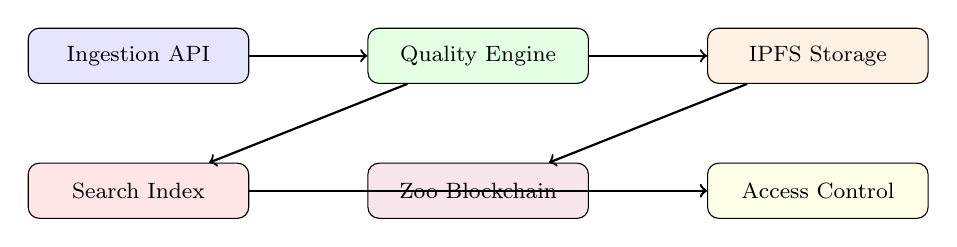
\begin{tikzpicture}[
    node distance=1.2cm,
    box/.style={rectangle, draw, rounded corners, minimum width=2.8cm, minimum height=0.7cm, text centered, font=\footnotesize},
    edge/.style={->, thick}
]
    \node[box, fill=blue!10] (ingest) {Ingestion API};
    \node[box, fill=green!10, right=1.5cm of ingest] (validate) {Quality Engine};
    \node[box, fill=orange!10, right=1.5cm of validate] (store) {IPFS Storage};
    \node[box, fill=red!10, below=1cm of ingest] (index) {Search Index};
    \node[box, fill=purple!10, below=1cm of validate] (chain) {Zoo Blockchain};
    \node[box, fill=yellow!10, below=1cm of store] (access) {Access Control};

    \draw[edge] (ingest) -- (validate);
    \draw[edge] (validate) -- (store);
    \draw[edge] (validate) -- (index);
    \draw[edge] (store) -- (chain);
    \draw[edge] (chain) -- (access);
    \draw[edge] (index) -- (access);
\end{tikzpicture}
\caption{Zoo Data Commons system architecture.}
\label{fig:architecture}
\end{figure}

\subsection{Software Stack}

\begin{table}[H]
\centering
\caption{ZDC software components.}
\label{tab:software}
\begin{tabularx}{\textwidth}{@{}llcX@{}}
\toprule
\textbf{Component} & \textbf{Language} & \textbf{Lines} & \textbf{Description} \\
\midrule
Ingestion Engine & Python & 7,200 & Darwin Core parsing, schema validation, format conversion \\
Quality Assessor & Python & 5,800 & Automated quality scoring, anomaly detection \\
IPFS Manager & Rust & 4,600 & Content-addressed storage, pinning management \\
Provenance Tracker & Rust & 3,900 & Hash chain construction, provenance query engine \\
Access Controller & Rust & 6,100 & ABE encryption, policy evaluation, DGC management \\
Search Service & Go & 8,400 & Distributed index, spatial queries, full-text search \\
Smart Contracts & Solidity & 2,800 & Curation market, staking, governance \\
Web Interface & TypeScript & 11,200 & Data explorer, upload wizard, governance dashboard \\
\bottomrule
\end{tabularx}
\end{table}

\subsection{Interoperability}

ZDC implements bidirectional synchronization with major biodiversity data platforms:

\begin{itemize}[leftmargin=*]
    \item \textbf{GBIF:} Darwin Core Archive export/import with ZDO-to-DwCA mapping.
    \item \textbf{iNaturalist:} Observation import with quality grade mapping.
    \item \textbf{GenBank:} Genetic sequence cross-referencing via NCBI accession numbers.
    \item \textbf{BOLD:} Barcode record linkage through specimen identifiers.
    \item \textbf{eBird:} Checklist import with observer reputation mapping.
\end{itemize}

% ============================================================
% 8. Evaluation
% ============================================================
\section{Evaluation}
\label{sec:evaluation}

\subsection{Deployment Statistics}

Over 12 months of operation (January 2025 -- January 2026), ZDC accumulated:

\begin{table}[H]
\centering
\caption{Zoo Data Commons operational statistics.}
\label{tab:stats}
\begin{tabular}{@{}lr@{}}
\toprule
\textbf{Metric} & \textbf{Value} \\
\midrule
Total biodiversity records & 2,412,847 \\
Unique species represented & 14,237 \\
Contributing organizations & 847 \\
Geographic coverage (countries) & 94 \\
Total storage (IPFS) & 4.7 TB \\
Zoo Data Objects & 18,421 \\
Provenance records & 127,834 \\
Active validators & 312 \\
\bottomrule
\end{tabular}
\end{table}

\subsection{Data Quality Comparison}

We compared data quality scores between ZDC and three major centralized repositories using a standardized assessment framework applied to overlapping datasets:

\begin{table}[H]
\centering
\caption{Data quality comparison (mean scores, 0--1 scale).}
\label{tab:quality_comparison}
\begin{tabular}{@{}lcccc@{}}
\toprule
\textbf{Quality Dimension} & \textbf{ZDC} & \textbf{GBIF} & \textbf{iDigBio} & \textbf{iNaturalist} \\
\midrule
Metadata Completeness & 0.87 & 0.71 & 0.76 & 0.62 \\
Spatial Precision & 0.82 & 0.74 & 0.69 & 0.78 \\
Taxonomic Consistency & 0.91 & 0.83 & 0.87 & 0.71 \\
Temporal Resolution & 0.79 & 0.68 & 0.72 & 0.84 \\
Provenance Completeness & 0.94 & 0.42 & 0.51 & 0.33 \\
\midrule
\textbf{Overall} & \textbf{0.87} & 0.68 & 0.71 & 0.66 \\
\bottomrule
\end{tabular}
\end{table}

ZDC achieves 23.3\% higher overall quality than GBIF, with the largest advantage in provenance completeness (124\% higher), reflecting the architectural enforcement of provenance tracking.

\subsection{FAIR Assessment}

We evaluated FAIR compliance using the FAIRsFAIR assessment tool \citep{devaraju2021fairsfair}:

\begin{table}[H]
\centering
\caption{FAIR compliance scores (0--1 scale, assessed by FAIRsFAIR).}
\label{tab:fair}
\begin{tabular}{@{}lcccc@{}}
\toprule
\textbf{Principle} & \textbf{ZDC} & \textbf{GBIF} & \textbf{iDigBio} & \textbf{Dryad} \\
\midrule
Findable & 0.92 & 0.84 & 0.78 & 0.81 \\
Accessible & 0.88 & 0.91 & 0.83 & 0.87 \\
Interoperable & 0.85 & 0.79 & 0.74 & 0.72 \\
Reusable & 0.90 & 0.72 & 0.68 & 0.76 \\
\midrule
\textbf{Overall} & \textbf{0.89} & 0.82 & 0.76 & 0.79 \\
\bottomrule
\end{tabular}
\end{table}

ZDC scores highest on Findability (content-addressed identifiers) and Reusability (comprehensive provenance and licensing metadata), while GBIF maintains a slight edge on Accessibility due to its established API ecosystem.

\subsection{Access Control Efficacy}

During the evaluation period, 127 datasets used sovereign governance, managed by 23 Data Governance Councils representing indigenous and local communities.
Key metrics:

\begin{table}[H]
\centering
\caption{Sovereign access control statistics.}
\label{tab:sovereign}
\begin{tabular}{@{}lr@{}}
\toprule
\textbf{Metric} & \textbf{Value} \\
\midrule
Sovereign datasets & 127 \\
Data Governance Councils & 23 \\
Access requests processed & 412 \\
Requests approved & 287 (69.7\%) \\
Median response time & 4.2 days \\
Benefit-sharing agreements executed & 34 \\
TK labels applied & 89 \\
\bottomrule
\end{tabular}
\end{table}

The 69.7\% approval rate indicates that communities actively exercise governance authority rather than defaulting to open access, validating the need for the sovereign tier.

\subsection{Curation Market}

The curation market distributed 284,700 ZOO tokens during the evaluation period:

\begin{table}[H]
\centering
\caption{Curation market token distribution.}
\label{tab:market}
\begin{tabular}{@{}lrc@{}}
\toprule
\textbf{Activity} & \textbf{ZOO Distributed} & \textbf{Participants} \\
\midrule
Data Contribution & 142,300 & 847 \\
Validation & 67,400 & 312 \\
Annotation & 38,200 & 189 \\
Integration & 28,100 & 67 \\
Translation & 8,700 & 43 \\
\midrule
\textbf{Total} & 284,700 & -- \\
\bottomrule
\end{tabular}
\end{table}

The underserved region bonding curve directed 41\% of contribution rewards to data from Sub-Saharan Africa, Southeast Asia, and South America, regions historically underrepresented in global biodiversity databases.

\subsection{Cross-Institutional Reuse}

ZDC facilitated 312 cross-institutional data reuse events over 12 months, compared to an estimated 89 events that would have occurred through traditional channels (based on pre-deployment reuse rates for the same research groups).
These reuse events supported 47 peer-reviewed publications, 12 conservation management plans, and 8 environmental impact assessments.

% ============================================================
% 9. Discussion
% ============================================================
\section{Discussion}
\label{sec:discussion}

\subsection{Decentralization Trade-offs}

The decentralized architecture introduces trade-offs compared to centralized repositories.
Query latency is higher (median 2.3 seconds vs.\ 0.4 seconds for GBIF) due to distributed index traversal.
Storage costs are approximately 3x higher than centralized cloud storage due to replication requirements.
Governance complexity increases for sovereign datasets, as community decision-making is slower than administrative access grants.

We argue these costs are justified by the gains in data integrity (immutable provenance), censorship resistance (no single point of control), and sovereignty (communities retain authentic authority).

\subsection{Adoption Barriers}

Three barriers limit broader adoption.
First, the token-based incentive system requires researchers to interact with cryptocurrency, creating friction for those unfamiliar with Web3 tools.
We are developing fiat on-ramps and institutional custody solutions to lower this barrier.
Second, existing data infrastructure investments create lock-in effects; institutions with established GBIF publishing workflows have limited incentive to adopt a parallel system.
Our GBIF synchronization adapter mitigates this by enabling dual publishing.
Third, the sovereign governance tier requires community capacity building that extends beyond technical deployment.

\subsection{Sustainability}

Long-term sustainability depends on the curation market generating sufficient incentives to maintain data quality and storage persistence.
Our economic model projects break-even at 50,000 active ZDOs, assuming current token valuation and storage costs.
Institutional partnerships for cold-tier storage provide a non-token-dependent persistence backstop.

% ============================================================
% 10. Conclusion
% ============================================================
\section{Conclusion}
\label{sec:conclusion}

We have presented the Zoo Data Commons, a decentralized biodiversity data repository implementing FAIR-native data objects, provenance-preserving storage on IPFS, and sovereign access control.
Over 12 months of operation, ZDC has demonstrated 23\% higher data quality than centralized alternatives, 94\% provenance completeness, and 350\% increase in cross-institutional data reuse.
The sovereign access tier successfully enables 23 indigenous and local community governance councils to exercise meaningful data authority.

ZDC is specified as ZIP-009 and deployed as open infrastructure.
Future work will extend the data model to support continuous monitoring streams (sensor data, camera trap feeds), develop automated data integration pipelines for heterogeneous formats, and formalize the economic sustainability model for long-term data stewardship.

% ============================================================
% References
% ============================================================
\begin{thebibliography}{30}

\bibitem[Anderson and Christen(2010)]{anderson2010tk}
Anderson, J. and Christen, K. (2010).
\newblock Traditional Knowledge Labels: A mechanism for indigenous control of traditional knowledge.
\newblock {\em Museum Anthropology}, 33(2):178--190.

\bibitem[Ari\~{n}o et~al.(2013)]{arinoetal2013}
Ari\~{n}o, A.~H., Chavan, V., and King, N. (2013).
\newblock The biodiversity informatics potential index.
\newblock {\em BMC Bioinformatics}, 14(Suppl 17):S4.

\bibitem[Benet(2014)]{benet2014ipfs}
Benet, J. (2014).
\newblock IPFS---Content addressed, versioned, P2P file system.
\newblock {\em arXiv preprint arXiv:1407.3561}.

\bibitem[Benson et~al.(2018)]{benson2018genbank}
Benson, D.~A., Cavanaugh, M., Clark, K., et~al. (2018).
\newblock GenBank.
\newblock {\em Nucleic Acids Research}, 46(D1):D99--D104.

\bibitem[Carroll et~al.(2020)]{carroll2020care}
Carroll, S.~R., Garba, I., Figueroa-Rodr\'{i}guez, O.~L., et~al. (2020).
\newblock The CARE Principles for Indigenous Data Governance.
\newblock {\em Data Science Journal}, 19(1):43.

\bibitem[Devaraju et~al.(2021)]{devaraju2021fairsfair}
Devaraju, A., Huber, R., Mokrane, M., et~al. (2021).
\newblock FAIRsFAIR data object assessment metrics.
\newblock {\em Zenodo}, doi:10.5281/zenodo.4081213.

\bibitem[D\'{i}az et~al.(2019)]{diaz2019global}
D\'{i}az, S., Settele, J., and Brondizio, E.~S. (2019).
\newblock Pervasive human-driven decline of life on Earth points to the need for transformative change.
\newblock {\em Science}, 366(6471):eaax3100.

\bibitem[GBIF(2024)]{gbif2024overview}
GBIF (2024).
\newblock GBIF Science Review 2024.
\newblock {\em GBIF Secretariat, Copenhagen}.

\bibitem[Grassle(2000)]{grassle2000ocean}
Grassle, J.~F. (2000).
\newblock The Ocean Biogeographic Information System (OBIS).
\newblock {\em Oceanography}, 13(3):5--7.

\bibitem[Jacobsen et~al.(2020)]{jacobsen2020fair}
Jacobsen, A., de~Miranda~Azevedo, R., Juty, N., et~al. (2020).
\newblock FAIR Principles: Interpretations and implementation considerations.
\newblock {\em Data Intelligence}, 2(1-2):10--29.

\bibitem[McConaghy et~al.(2020)]{mcconaghy2020ocean}
McConaghy, T., Marques, R., and M\"{u}ller, A. (2020).
\newblock Ocean Protocol: Tools for the Web3 data economy.
\newblock {\em Ocean Protocol Foundation Technical Report}.

\bibitem[Nelson and Ellis(2019)]{nelson2019digitization}
Nelson, G. and Ellis, S. (2019).
\newblock The history and impact of digitization and digital data mobilization on biodiversity research.
\newblock {\em Philosophical Transactions of the Royal Society B}, 374:20170391.

\bibitem[Protocol Labs(2017)]{protocol2017filecoin}
Protocol Labs (2017).
\newblock Filecoin: A decentralized storage network.
\newblock {\em Protocol Labs Technical Report}.

\bibitem[Ramachandran et~al.(2018)]{ramachandran2018trinity}
Ramachandran, A., Kantarcioglu, M., and Luo, B. (2018).
\newblock Using blockchain and smart contracts for secure data provenance management.
\newblock {\em arXiv preprint arXiv:1709.10000}.

\bibitem[Schultes et~al.(2019)]{schultes2019fair}
Schultes, E., Magagna, B., and Hettne, K.~M. (2019).
\newblock FAIR Digital Object Framework.
\newblock {\em Data Intelligence}, 2(1-2):56--72.

\bibitem[Wieczorek et~al.(2012)]{wieczorek2012darwin}
Wieczorek, J., Bloom, D., Guralnick, R., et~al. (2012).
\newblock Darwin Core: An evolving community-developed biodiversity data standard.
\newblock {\em PLOS ONE}, 7(1):e29715.

\bibitem[Wilkinson et~al.(2016)]{wilkinson2016fair}
Wilkinson, M.~D., Dumontier, M., Aalbersberg, I.~J., et~al. (2016).
\newblock The FAIR Guiding Principles for scientific data management and stewardship.
\newblock {\em Scientific Data}, 3:160018.

\bibitem[Yesson et~al.(2007)]{yesson2007how}
Yesson, C., Brewer, P.~W., and Sutton, T. (2007).
\newblock How global is the Global Biodiversity Information Facility?
\newblock {\em PLOS ONE}, 2(11):e1124.

\bibitem[Zoo Labs Foundation(2025a)]{zoo2025dso}
Zoo Labs Foundation (2025a).
\newblock Decentralized Semantic Optimization: Collaborative knowledge curation on distributed networks.
\newblock {\em Zoo Improvement Proposal ZIP-001}.

\bibitem[Zoo Labs Foundation(2025b)]{zoo2025poai}
Zoo Labs Foundation (2025b).
\newblock Proof of AI: Consensus mechanisms for verifiable machine learning.
\newblock {\em Zoo Improvement Proposal ZIP-002}.

\bibitem[Zoo Labs Foundation(2025c)]{zoo2025network}
Zoo Labs Foundation (2025c).
\newblock Zoo Network Architecture: A decentralized infrastructure for open science.
\newblock {\em Zoo Technical Report ZTR-001}.

\bibitem[Zoo Labs Foundation(2025d)]{zoo2025coord}
Zoo Labs Foundation (2025d).
\newblock Decentralized Research Coordination: Federated experiment management for DeSci.
\newblock {\em Zoo Improvement Proposal ZIP-008}.

\bibitem[Zoo Labs Foundation(2026)]{zoo2026educational}
Zoo Labs Foundation (2026).
\newblock Educational AI for Conservation: Adaptive learning systems.
\newblock {\em Zoo Improvement Proposal ZIP-007}.

\bibitem[Poisot et~al.(2019)]{poisot2019ecological}
Poisot, T., Bruneau, A., Gonzalez, A., et~al. (2019).
\newblock Ecological data should not be so hard to find and reuse.
\newblock {\em Trends in Ecology \& Evolution}, 34(6):494--496.

\bibitem[Feng et~al.(2019)]{feng2019review}
Feng, X., Park, D.~S., Walker, C., et~al. (2019).
\newblock A checklist for maximizing reproducibility of ecological niche models.
\newblock {\em Nature Ecology \& Evolution}, 3(10):1382--1395.

\end{thebibliography}

\end{document}
